% ===========================================================================
%  Purification of Noisy Bell States
%  Noise Thresholds - Physical and Virtual Protocols - Repeated Dynamics
%
%  Build:  latexmk -pdf pqec_thresholds.tex
% ===========================================================================
\documentclass[aspectratio=169,10pt,t]{beamer}

\usepackage[T1]{fontenc}
\usepackage[utf8]{inputenc}
\usepackage[scaled=0.94]{helvet}
\renewcommand{\familydefault}{\sfdefault}
\usepackage{amsmath,amssymb,bm}
\usepackage{booktabs}
\usepackage{array}
\usepackage{graphicx}
\usepackage{microtype}

\usepackage{beamerthemeqitwhite}

\hypersetup{pdftitle={Purification of Noisy Bell States},
            pdfauthor={Jaehun Han}}

% ---- spacing ---------------------------------------------------------------
\setlength{\parskip}{0pt}
\renewcommand{\arraystretch}{1.12}
\setlength{\tabcolsep}{4.5pt}
\newcommand{\rowgap}{\addlinespace[1.2pt]}
\setlength{\abovedisplayskip}{3pt plus 1pt minus 1pt}
\setlength{\belowdisplayskip}{3pt plus 1pt minus 1pt}
\setlength{\abovedisplayshortskip}{1pt}
\setlength{\belowdisplayshortskip}{2pt}

% ---- shorthands ------------------------------------------------------------
\newcommand{\ket}[1]{\lvert #1 \rangle}
\newcommand{\bra}[1]{\langle #1 \rvert}
\newcommand{\ketbra}[2]{\lvert #1 \rangle\langle #2 \rvert}
\newcommand{\avg}[1]{\langle #1 \rangle}
\newcommand{\Tr}{\operatorname{Tr}}
\newcommand{\Phip}{\Phi^{+}}
\newcommand{\qb}{\bar{q}}
\newcommand{\acc}[1]{{\color{qitaccent}#1}}
\newcommand{\warn}[1]{{\color{qitwarn}#1}}
\newcommand{\gry}[1]{{\color{qitink2}#1}}
\newcommand{\unit}[1]{{\color{qitgray}#1}}
\newcommand{\stat}[1]{{\scriptsize\color{qitgray}\textsc{#1}}}

\title{Purification of Noisy Bell States}
\subtitle{Noise Thresholds \quad$\cdot$\quad Physical and Virtual Protocols
          \quad$\cdot$\quad Repeated Dynamics}
\author{Jaehun Han}
\institute{QIT Lab}
\date{2026.10.12}

\begin{document}

% ===========================================================================
\begin{frame}[plain]
  \vspace{0.26\paperheight}
  {\usebeamerfont{title}\usebeamercolor[fg]{title}\inserttitle\par}
  \vspace{1.2ex}
  {\color{qitrule}\rule{0.40\paperwidth}{1.2pt}}\par
  \vspace{1.8ex}
  {\usebeamerfont{subtitle}\usebeamercolor[fg]{subtitle}\insertsubtitle\par}
  \vspace{0.21\paperheight}
  {\usebeamerfont{author}\usebeamercolor[fg]{author}%
   \insertdate\quad Jaehun Han, QIT Lab\par}
\end{frame}

% ===========================================================================
\begin{frame}{Outline}
  \vspace{1.5ex}
  \begin{columns}[T,onlytextwidth]
  \begin{column}{0.47\textwidth}\vspace{0pt}
    \small
    \begin{enumerate}\itemsep0.80ex
      \item Research motivation
      \item Three protocols: 4Q, 5Q, 6Q
      \item Ideal purification
      \item Noisy implementation
      \item Circuit decompositions
      \item Equivalence of the 5Q and 6Q estimators
    \end{enumerate}
  \end{column}
  \begin{column}{0.47\textwidth}\vspace{0pt}
    \small
    \begin{enumerate}\itemsep0.80ex
      \setcounter{enumi}{6}
      \item Exact Bell-diagonal maps
      \item Repeated dynamics and fixed points
      \item Resource comparison
      \item Operational thresholds: five definitions
      \item Threshold results
      \item Discussion and next steps
    \end{enumerate}
  \end{column}
  \end{columns}
  \vfill
  {\footnotesize\color{qitgray}
   Every number is reproduced by executed code; each claim is labelled
   \textsc{proved}, \textsc{numerical} or \textsc{open}.}
  \vspace{1ex}
\end{frame}

% ===========================================================================
% 1. Research motivation
% ===========================================================================
\begin{frame}{1 \quad Research motivation}{When does an \emph{imperfect} purifier still help?}
  \footnotesize
  \vspace{0.6ex}
  \begin{columns}[T,onlytextwidth]
  \begin{column}{0.50\textwidth}\vspace{0pt}
    \textbf{The primitive.}\; Purification maps
    \[
      \mathcal{P}(\rho)=\frac{\rho^{2}}{\Tr\rho^{2}},
    \]
    concentrating weight on the dominant eigenvector and removing the
    leading error of a noisy Bell pair.
    \medskip

    \textbf{Two ways to use it.}
    \begin{itemize}\itemsep0.45ex
      \item \acc{Physical} --- a genuine state is produced on a postselected
            branch.\; Cost: $P_{\mathrm{succ}}<1$.
      \item \acc{Virtual} (VD / PQEC) --- only
            $\avg{O}_{\mathcal{P}}=\Tr(O\rho^{2})/\Tr\rho^{2}$ is estimated;
            the purified state is \emph{never prepared}.\; Cost: sampling
            overhead.
    \end{itemize}
  \end{column}
  \begin{column}{0.46\textwidth}\vspace{0pt}
    \textbf{Where the literature stops.}\\[0.3ex]
    Raghoonanan \& Byrnes, \emph{Quantum Error Correction by Purification},
    arXiv:2603.11568 (2026): noise on the \emph{data}, purification gadget
    assumed \emph{perfect}.
    \medskip

    \textbf{This project.}\\[0.3ex]
    Put the noise \emph{inside the purifier} --- on the Fredkin gates at the
    heart of the SWAP test --- and ask how large the per-gate error may be
    before purification stops being useful.
    \medskip

    \centerline{\fbox{\parbox{0.90\linewidth}{\centering
      \textbf{operational threshold}\\[0.3ex]
      \unit{the largest per-CNOT noise $q$ at which the protocol still does
      what it promises}}}}
  \end{column}
  \end{columns}
  \vfill
  {\footnotesize Input family throughout --- Bell-isotropic:
   $\rho(\varepsilon)=(1-\varepsilon)\ketbra{\Phip}{\Phip}+\varepsilon I/4$,\;
   $F_{0}=1-\tfrac{3}{4}\varepsilon$,\; entangled iff $\varepsilon<2/3$.}
  \vspace{0.6ex}
\end{frame}

% ===========================================================================
% 2. Three protocols
% ===========================================================================
\begin{frame}{2 \quad Three protocols}{4Q global \quad$\cdot$\quad 5Q quantum communication \quad$\cdot$\quad 6Q LOCC}
  \vspace{0.6ex}
  \begin{columns}[T,onlytextwidth]
    \begin{column}{0.325\textwidth}\centering
      {\footnotesize\textbf{4Q} \,\unit{postselected comparator}}\\[0.5ex]
      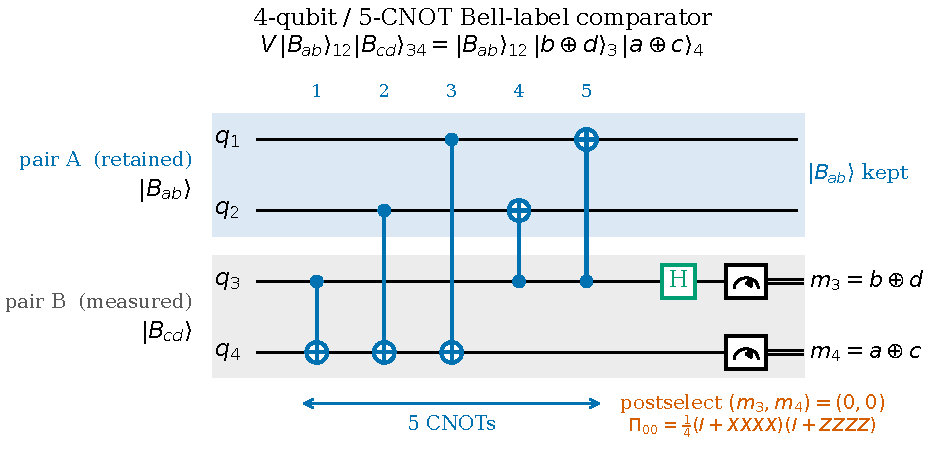
\includegraphics[width=\linewidth,height=0.295\paperheight,keepaspectratio]{figures/4q_circuit.pdf}
    \end{column}
    \begin{column}{0.325\textwidth}\centering
      {\footnotesize\textbf{5Q} \,\unit{SWAP-test PQEC}}\\[0.5ex]
      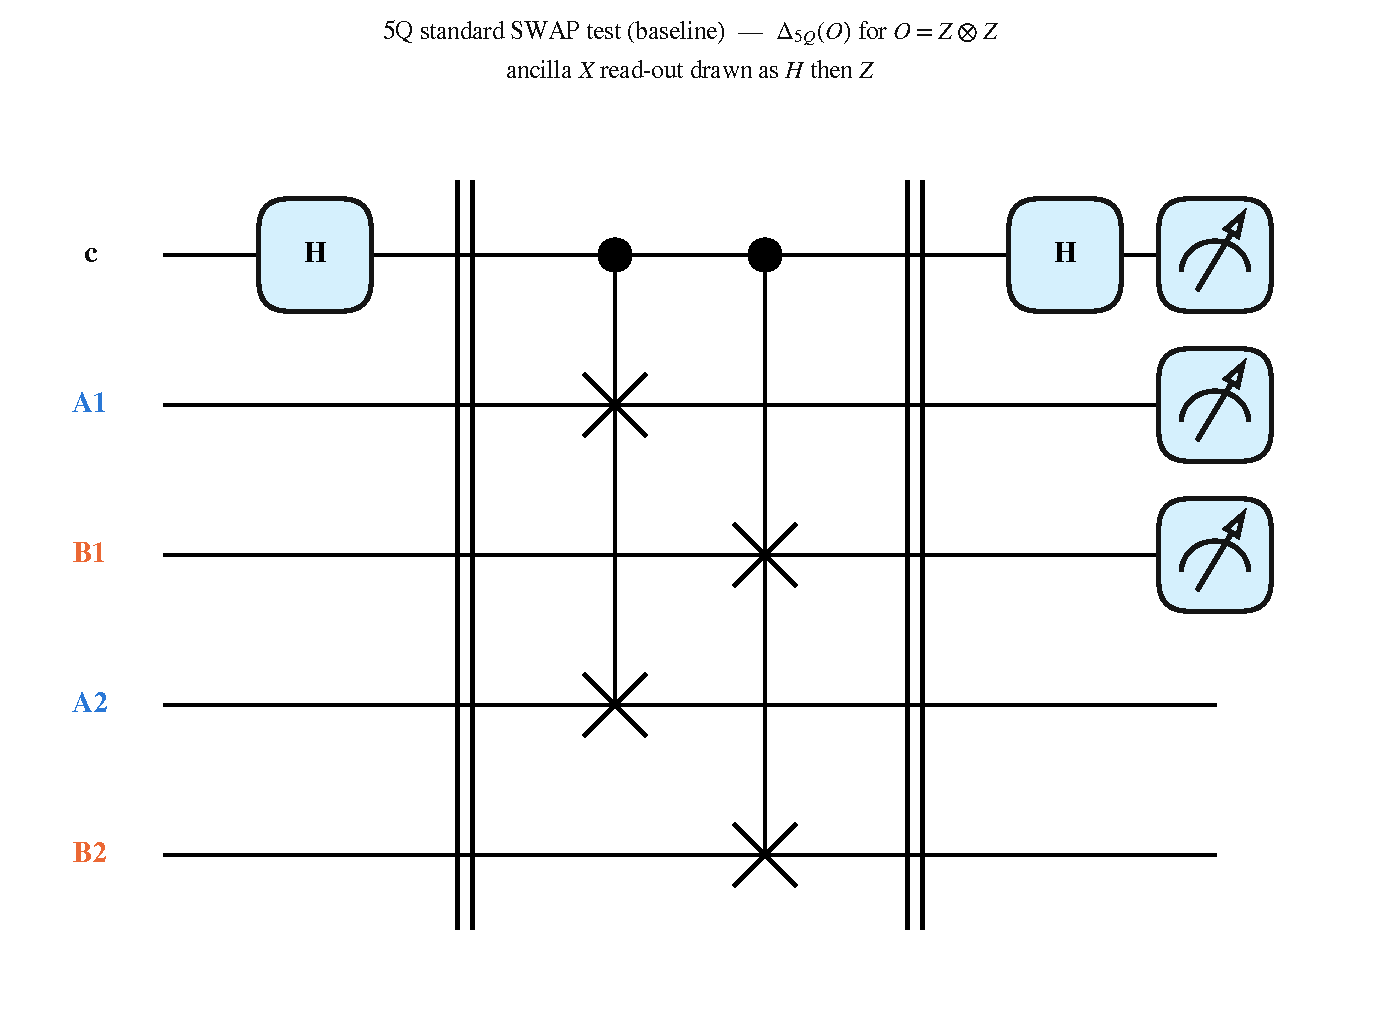
\includegraphics[width=\linewidth,height=0.295\paperheight,keepaspectratio]{figures/5q_circuit.pdf}
    \end{column}
    \begin{column}{0.325\textwidth}\centering
      {\footnotesize\textbf{6Q} \,\unit{distributed LOCC-VD}}\\[0.5ex]
      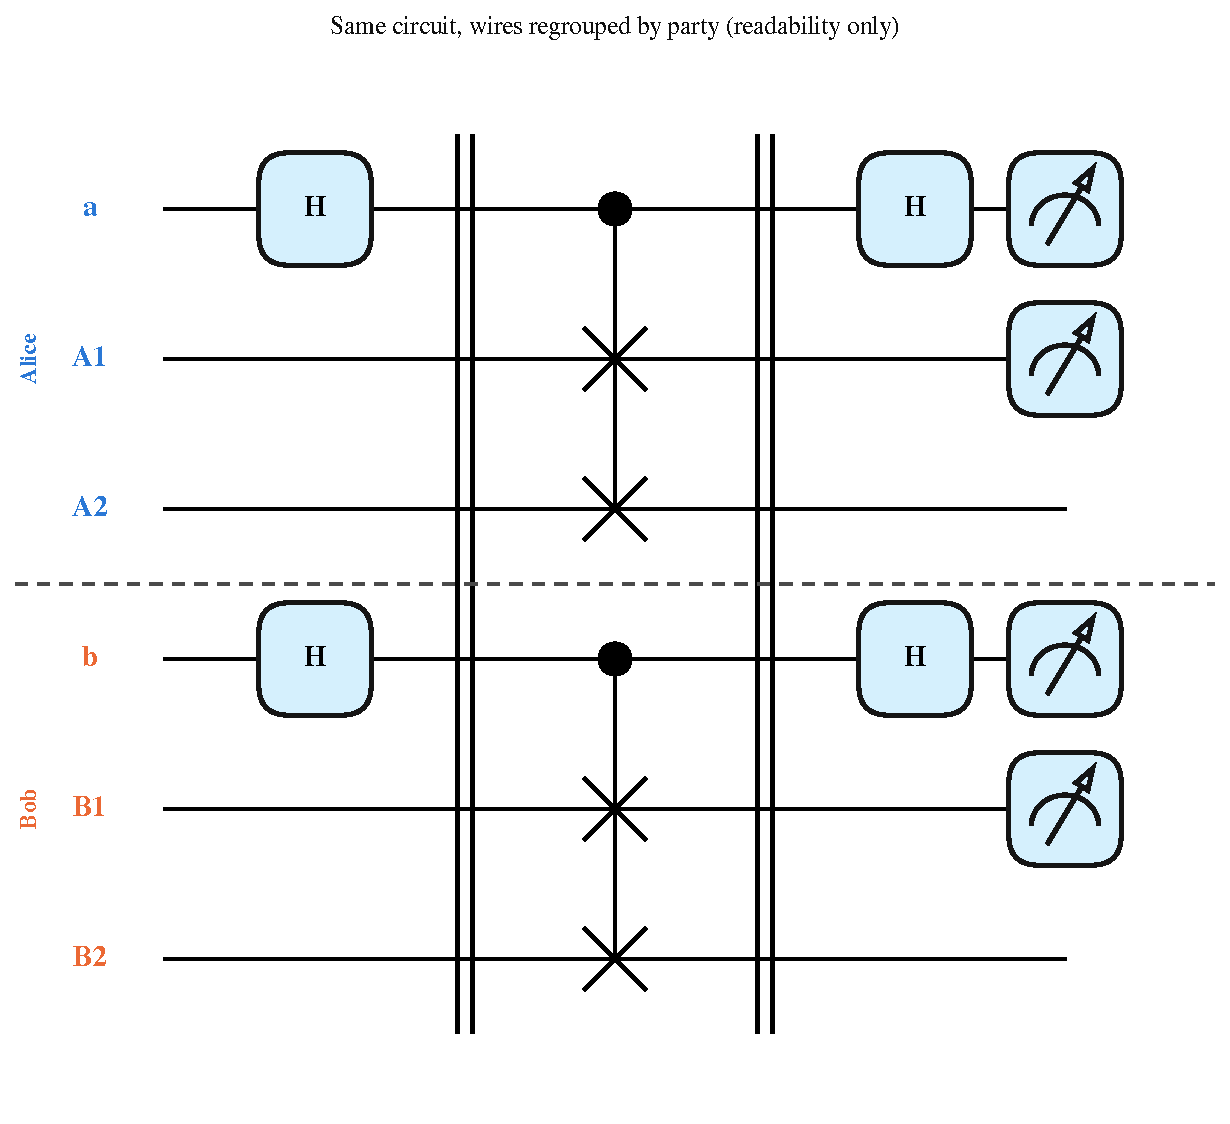
\includegraphics[width=\linewidth,height=0.295\paperheight,keepaspectratio]{figures/6q_circuit.pdf}
    \end{column}
  \end{columns}
  \vspace{1.6ex}
  \centering\footnotesize\setlength{\tabcolsep}{4pt}
  \begin{tabular}{@{}l l l l l l@{}}
    \toprule
     & qubits & ancillas & gates across the $A|B$ cut & output & per-round cost\\
    \midrule
    \textbf{4Q} & 4 & --- & \warn{3 of 5 CNOTs cross}      & a physical state   & $P_{\mathrm{succ}}=\Tr\rho^{2}$\\\rowgap
    \textbf{5Q} & 5 & 1 shared & one ancilla must meet \emph{both} copies & an expectation value & sampling overhead\\\rowgap
    \textbf{6Q} & 6 & 1 per party & \acc{none --- strictly local} & an expectation value & sampling overhead\\
    \bottomrule
  \end{tabular}
  \vfill
  \raggedright\footnotesize
  4Q needs \emph{global} operations on one processor;\; 5Q needs a shared
  ancilla, i.e.\ \emph{quantum communication};\; 6Q is \emph{LOCC} --- local
  Fredkins plus classical post-processing.
  \vspace{0.5ex}
\end{frame}

% ===========================================================================
% 3. Ideal purification
% ===========================================================================
\begin{frame}{3 \quad Ideal purification}{All three read the same object $\rho^{2}$ --- but hand back different things}
  \vspace{0.6ex}
  \scriptsize
  \setlength{\tabcolsep}{4pt}\begin{tabular}{@{}p{0.055\textwidth} p{0.505\textwidth} p{0.34\textwidth}@{}}
    \toprule
    & \textbf{what the circuit computes} & \textbf{what you get}\\
    \midrule
    \textbf{4Q}
      & $K_{00}=\sum_{i}\ketbra{B_i}{B_i}\otimes\bra{B_i}$: an
        \emph{elementwise (Schur) square} in the Bell basis, $=\rho^{2}$
        for Bell-diagonal $\rho$
      & \acc{a physical state}
        $\rho_{\mathrm{out}}=\rho^{2}/\Tr\rho^{2}$ on the $(0,0)$ branch,
        $P_{\mathrm{succ}}=\Tr\rho^{2}$\\\rowgap
    \textbf{5Q}
      & $\avg{Z_a\otimes O}/\avg{Z_a\otimes I}=\Tr(O\rho^{2})/\Tr\rho^{2}$
      & \acc{a number only}; the reduced state is \emph{not}
        $\rho^{2}/\Tr\rho^{2}$\\\rowgap
    \textbf{6Q}
      & $\Delta(O)=\avg{X_aX_b\otimes O}-\avg{Y_aY_b\otimes O}=\Tr(O\rho^{2})$,
        hence $T_{6Q}=\tfrac14\sum_{P}\Delta(P)\,P=\rho^{2}$
      & \acc{a number only}; no postselection, every shot kept\\
    \bottomrule
  \end{tabular}

  \vspace{2.0ex}
  \footnotesize
  \begin{columns}[T,onlytextwidth]
  \begin{column}{0.47\textwidth}\vspace{0pt}
    \textbf{Bell-isotropic input, ideal circuit}
    \[
      \varepsilon'=\frac{\varepsilon^{2}}{4-6\varepsilon+3\varepsilon^{2}},
      \qquad
      P_{\mathrm{succ}}=\frac{4-6\varepsilon+3\varepsilon^{2}}{4}
    \]
    \smallskip
    Circuit vs.\ independent analytics, 501 sweep points:
    agreement \acc{$7.8\times10^{-16}$}.\; \stat{proved + verified}
  \end{column}
  \begin{column}{0.49\textwidth}\vspace{0pt}
    \textbf{Two caveats that matter later}
    \begin{itemize}\itemsep0.35ex
      \item the $\rho^{2}$ identity for 4Q holds \emph{only} for
            Bell-diagonal $\rho$ --- otherwise a Schur square (differs by
            ${>}10^{-6}$ on 40 random states);
      \item 4Q is \emph{not} LOCC, which is why it can re-entangle a
            separable input for
            $2/3\le\varepsilon<2-2\sqrt3/3\approx0.8453$.
    \end{itemize}
  \end{column}
  \end{columns}
\end{frame}

% ===========================================================================
% 4. Noisy implementation
% ===========================================================================
\begin{frame}{4 \quad Noisy implementation}{Why the gate decomposition becomes part of the physics}
  \footnotesize
  \vspace{0.6ex}
  \begin{columns}[T,onlytextwidth]
  \begin{column}{0.46\textwidth}\vspace{0pt}
    \textbf{Noise model, identical everywhere.}\\[0.3ex]
    A two-qubit \emph{replacement} depolarizing channel after \emph{every}
    CNOT, on exactly that CNOT's wires:
    \[
      \mathcal{D}^{(ij)}_{q}(\sigma)=(1-q)\,\sigma
        + q\Bigl[\tfrac{I_{ij}}{4}\otimes\Tr_{ij}\sigma\Bigr],
      \quad \qb:=1-q .
    \]
    Single-qubit gates, preparation, measurement and classical
    post-processing stay ideal.\; $q=0$ is the exact identity; $q=1$ leaves
    the pair exactly $I/4$.
    \medskip

    In the Heisenberg picture the adjoint is trivial on Pauli strings ---
    $\mathcal{D}^{\dagger}(P)=P$ when $P_i=P_j=I$, else $\qb P$ --- which is
    what makes the closed forms on slide 7 possible.
  \end{column}
  \begin{column}{0.50\textwidth}\vspace{0pt}
    \textbf{A negative result that forced this model.}\\[0.3ex]
    Depolarize at the \emph{Fredkin} level instead ($g_F$ on the three
    touched qubits):
    \[
      F_{\mathrm{PQEC}}(p,g_F)=\frac{(1+3\alpha^{2})^{2}}{4(1+3\alpha^{4})}
        = F_{\mathrm{ideal}}(p),\quad \alpha^{2}=1-\varepsilon .
    \]
    \warn{The threshold disappears.}\; Both parity correlators shrink by the
    same $(1-g_F)^{2}$, so the ratio is unchanged for every $g_F<1$; the
    only cost is sampling, $N\sim(1-g_F)^{-4}$. \stat{verified to $10^{-13}$}
    \medskip

    \textbf{Lesson.}\; A real operational threshold needs noise that damps
    numerator and denominator \emph{asymmetrically} --- i.e.\ noise attached
    to the \emph{decomposed} gates.
    \smallskip

    $\Rightarrow$ the CNOT decomposition is no longer a compilation detail.
    \acc{It changes the channel.}
  \end{column}
  \end{columns}
\end{frame}

% ===========================================================================
% 5. Circuit decompositions
% ===========================================================================
\begin{frame}{5 \quad Circuit decompositions}{Same ideal unitary $U_{\mathrm{PQEC}}=H_a\,\mathrm{CSWAP}\,\mathrm{CSWAP}\,H_a$, three different channels}
  \vspace{0.8ex}
  \scriptsize
  \begin{tabular}{@{}l p{0.42\textwidth} c c l@{}}
    \toprule
    \textbf{5Q} & construction & CNOTs & Bell-diagonal sector & one-round loss\\
    \midrule
    Type 3 & textbook $\mathrm{CSWAP}=\mathrm{CNOT}\cdot\mathrm{Toffoli}\cdot
             \mathrm{CNOT}$ with a Clifford$+T$ Toffoli: 8 CNOT per Fredkin
           & \textbf{16} & \acc{exactly invariant} & $F_1=1-\tfrac{17}{8}q+O(q^{2})$\\\rowgap
    Type 4 & Qiskit / pytket peephole resynthesis of the \emph{same}
             unitary; $14=2\times7$, optimal per Fredkin
           & \textbf{14} & \acc{exactly invariant} & $F_1=1-\tfrac{7}{4}q+O(q^{2})$\\\rowgap
    Type 5 & gauge-matched ring ansatz learned to $3\times10^{-15}$ at
             $L{=}3$ (18 CNOT), greedy-pruned to 14; \textbf{13 unreachable}
           & \textbf{14} & \warn{broken at $O(q)$} & $F_1=1-\tfrac{5}{4}q+O(q^{2})$\\
    \bottomrule
  \end{tabular}

  \vspace{2.4ex}
  \begin{columns}[T,onlytextwidth]
  \begin{column}{0.445\textwidth}\vspace{0pt}
    \footnotesize
    \textbf{The distributed 6Q versions}
    \begin{itemize}\itemsep0.25ex
      \item \textbf{6Q-L16} from Type 3: $8+8$ CNOTs, \acc{0 cross-party};
            each Fredkin is already local.
      \item \textbf{6Q-L14} from Type 4: $7+7$ CNOTs, \acc{0 cross-party},
            but locality is \emph{not} manifest.
    \end{itemize}
    \smallskip
    \textbf{Type-4 factorisation.} \stat{verified}\;
    14 CNOTs split $7+7$ by \textbf{18 disjoint-support moves}; the blocks
    are gate-for-gate identical and
    $U_{G7}=e^{-i\pi/8}\mathrm{Fredkin}$ to $7.0\times10^{-16}$.
    \unit{Without the phase the residual is $0.39$.}
  \end{column}
  \begin{column}{0.525\textwidth}\vspace{0pt}
    \centering
    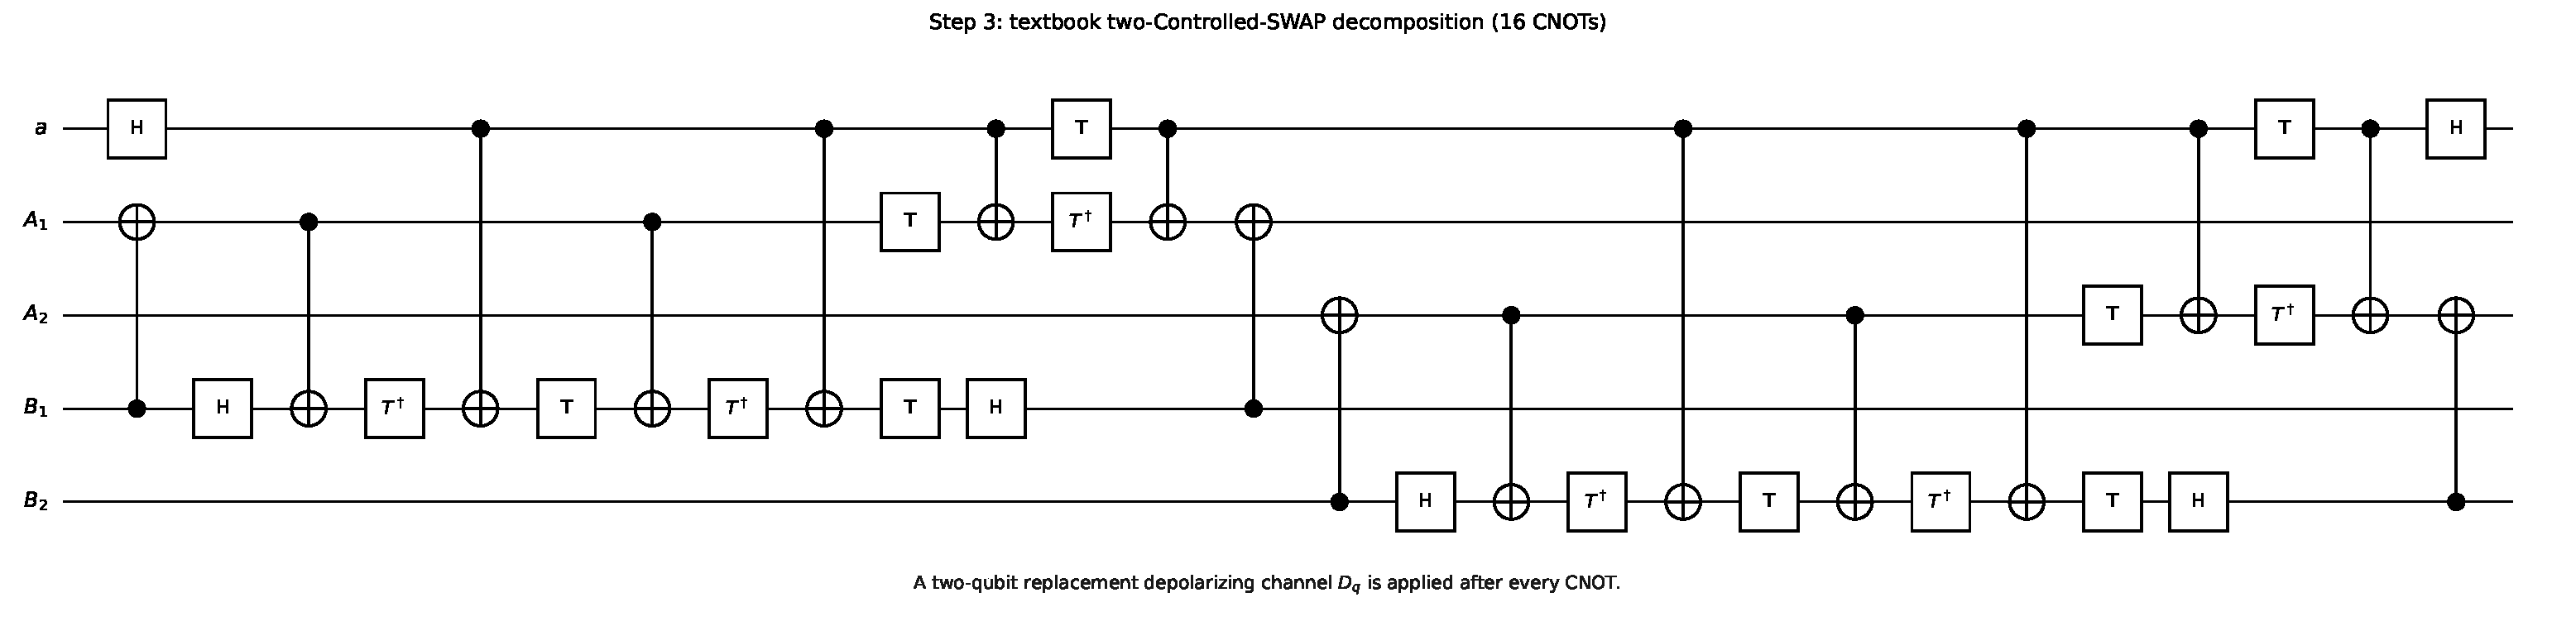
\includegraphics[width=\linewidth]{figures/type3_16cnot.pdf}\\[0.4ex]
    {\scriptsize\color{qitgray}Type 3: the 16-CNOT round, with a
     depolarizing channel after every CNOT.}
  \end{column}
  \end{columns}
\end{frame}

% ===========================================================================
% 6. Equivalence
% ===========================================================================
\begin{frame}{6 \quad Equivalence of the 5Q and 6Q estimators}{The LOCC protocol computes exactly what the shared-ancilla protocol computes}
  \footnotesize
  \vspace{0.6ex}
  \begin{columns}[T,onlytextwidth]
  \begin{column}{0.46\textwidth}\vspace{0pt}
    \textbf{Ideal case.} \stat{proved}\;
    With $S=S_AS_B$ and $R$ \emph{any} four-qubit input,
    \[
      \underbrace{C_{XX}(O)-C_{YY}(O)}_{\text{6Q}}
        =\tfrac12\Tr\!\bigl[\bar O\,(RS+SR)\bigr]
        =\underbrace{\avg{X_c\otimes\bar O}}_{\text{5Q}} .
    \]
    \emph{Mechanism:}
    $X\!\otimes\!X-Y\!\otimes\!Y=2(\ketbra{00}{11}+\ketbra{11}{00})$, so the
    $S_A\!\leftrightarrow\!S_B$ coherences cancel and only the ``neither
    swapped'' $\leftrightarrow$ ``both swapped'' interference survives ---
    precisely the single-ancilla SWAP interference.
    \smallskip

    For $R=\rho\otimes\rho$ this is $\Tr(O\rho^{2})$; with $O=I$, the purity.
  \end{column}
  \begin{column}{0.50\textwidth}\vspace{0pt}
    \textbf{Noisy case --- proved as well.} \stat{proved}\\[0.4ex]
    $\Delta_5(O;R)=\Delta_6(O;R)$ \emph{exactly}, for every $q\in[0,1]$,
    every four-qubit $R$ and every Hermitian $O$ --- Type 3 and Type 4
    alike. The raw, unnormalised check:
    \smallskip

    \centering\scriptsize
    \begin{tabular}{@{}l c c@{}}
      \toprule
       & Type 3 / 6Q-L16 & Type 4 / 6Q-L14\\
      \midrule
      comparisons                & 97\,440 & 97\,440\\\rowgap
      $\max|\Delta_5-\Delta_6|$  & \acc{$7.77\times10^{-16}$} & \acc{$5.55\times10^{-16}$}\\\rowgap
      mean                       & $2.1\times10^{-17}$ & $1.5\times10^{-17}$\\\rowgap
      $\Delta_5(I)$ vs $\Delta_6(I)$ & $7.8\times10^{-16}$ & $4.4\times10^{-16}$\\\rowgap
      $|\Omega_5-2\Omega_6|$     & $2.8\times10^{-16}$ & $1.7\times10^{-16}$\\\rowgap
      negative controls          & $\ge4.8\times10^{-4}$ & $\ge5.3\times10^{-4}$\\
      \bottomrule
    \end{tabular}
    \smallskip

    \raggedright
    94 two-qubit states $\times$ 56 observables $\times$ 15 values of
    $q\in[0,1]$, plus 22 \emph{arbitrary} four-qubit inputs $R$ --- the
    equality does not need two identical copies.
  \end{column}
  \end{columns}
  \vfill
  {\footnotesize
   \textbf{Consequence.}\; The quantum-communication protocol (5Q) and the
   LOCC protocol (6Q) are \acc{the same estimator under the same noise}.
   Going LOCC costs one extra ancilla and removes every cross-party
   two-qubit gate --- at no statistical cost.}
  \vspace{0.4ex}
\end{frame}

% ===========================================================================
% 7. Exact maps
% ===========================================================================
\begin{frame}{7 \quad Exact Bell-diagonal maps}{Noisy one-round map on $\rho=\tfrac14(II+xXX+yYY+zZZ)$, with $\qb=1-q$}
  \scriptsize
  \vspace{1.0ex}
  \begin{columns}[T,onlytextwidth]
  \begin{column}{0.465\textwidth}\vspace{0pt}
    \textbf{4Q postselected} (5 CNOTs)\; \stat{proved}
    \begin{align*}
      D &= 1+\qb^{5}(x^{2}+y^{2})+\qb^{3}z^{2},\qquad
      P_{\mathrm{succ}}=\tfrac{D}{4}\\[0.2ex]
      x' &= \qb^{3}\bigl[(1+\qb)x-2\qb^{2}yz\bigr]/D\\
      y' &= \qb^{4}\bigl[(1+\qb)y-2\qb\,xz\bigr]/D\\
      z' &= \qb^{4}\bigl[(1+\qb)z-2\qb\,xy\bigr]/D
    \end{align*}
    Invariant plane $y=-z$; Bell-isotropic inputs stay on it. Matches the
    dense simulator to $4.4\times10^{-16}$.
    \smallskip

    \textbf{Off-Bell sector.}\; The exact $15\times15$ Jacobian at the fixed
    point has \acc{all twelve off-Bell eigenvalues zero} --- coherences enter
    only at second order, $\delta\to\delta^{2}$. A full-state attractor, not
    a saddle.
  \end{column}
  \begin{column}{0.50\textwidth}\vspace{0pt}
    \textbf{5Q Type 3 / 6Q-L16} (16 CNOTs)\; \stat{proved}
    \begin{gather*}
      D_{3}=1+\qb^{4}(x^{2}+y^{2}+z^{2})\\
      x'=\tfrac{2\qb^{6}(x-yz)}{D_{3}},\quad
      y'=\tfrac{2\qb^{6}(y-xz)}{D_{3}},\quad
      z'=\tfrac{\qb^{5}(1+\qb)(z-xy)}{D_{3}}
    \end{gather*}
    \textbf{5Q Type 4 / 6Q-L14} (14 CNOTs) --- same structure, shallower
    exponents:
    \begin{gather*}
      D_{4}=1+\qb^{2}(x^{2}+y^{2}+z^{2})\\
      x'=\tfrac{2\qb^{4}(x-yz)}{D_{4}},\quad
      y'=\tfrac{2\qb^{4}(y-xz)}{D_{4}},\quad
      z'=\tfrac{\qb^{3}(1+\qb)(z-xy)}{D_{4}}
    \end{gather*}
    \smallskip
    Both map $\mathcal{S}_{\mathrm{BD}}\to\mathcal{S}_{\mathrm{BD}}$
    \acc{exactly}; the plane $y=-x$ is invariant, so $u=x=-y$, $v=z$ suffice
    and $F=(1+2u+v)/4$. At $q=0$ every map reduces to $\rho^{2}/\Tr\rho^{2}$.
    \smallskip

    \warn{Type 5 does not close:} one round on a Bell-diagonal input puts
    $O(q)$ weight on $XY\!-\!YX$, $XZ\!+\!ZX$, $YZ\!-\!ZY$ --- all 15 Pauli
    coordinates must be tracked.
  \end{column}
  \end{columns}
\end{frame}

% ===========================================================================
% 8. Repeated dynamics
% ===========================================================================
\begin{frame}{8 \quad Repeated dynamics}{$\rho_{n+1}=M_q(\rho_n)$ --- bilinear in $\rho$, nonlinear through the normalisation}
  \vspace{0.8ex}
  \begin{columns}[T,onlytextwidth]
  \begin{column}{0.50\textwidth}\vspace{0pt}
    \scriptsize
    \begin{tabular}{@{}l c c c@{}}
      \toprule
       & \textbf{Type 3} & \textbf{Type 4} & \textbf{4Q}\\
      \midrule
      CNOTs & 16 & 14 & 5\\\rowgap
      $F_\star$ to $O(q)$
        & $1-\tfrac{17}{8}q$ & $1-\tfrac{7}{4}q$ & $1-q$\\\rowgap
      next order
        & $-\tfrac{247}{64}q^{2}$ & $-\tfrac{23}{16}q^{2}$ & $-\tfrac{23}{8}q^{2}$\\\rowgap
      $q_{\mathrm{SN}}$ \unit{(fixed point exists)}
        & 0.130579 & \acc{0.189417} & 0.180670\\\rowgap
      $q_{\mathrm{ent}}$ \unit{($F_\star=1/2$)}
        & 0.129137 & \acc{0.184736} & 0.179815\\\rowgap
      Bell-diagonal closure & yes & yes & yes\\
      \bottomrule
    \end{tabular}
    \medskip

    Between $q_{\mathrm{ent}}$ and $q_{\mathrm{SN}}$ the attractor exists but
    is already \emph{separable}; above $q_{\mathrm{SN}}$ every Bell-isotropic
    input decays to $I/4$.
    \medskip

    \textbf{Type 5 is qualitatively different.}\;
    At $\bar\varepsilon=0.9$, $q=0.01$: $F_{10}\approx F_{500}\approx0.987$,
    then $F_{1000}\approx0.544$, $F_{5000}\approx0.408$ --- a metastable
    plateau, then escape ($\max|\lambda(J_{\mathrm{full}})|\approx1.0116>1$)
    to a \emph{product fixed circle}: purity $(1-q/2)^{2}\to1$, but
    concurrence and negativity \acc{exactly zero}.
  \end{column}
  \begin{column}{0.465\textwidth}\vspace{0pt}
    \centering
    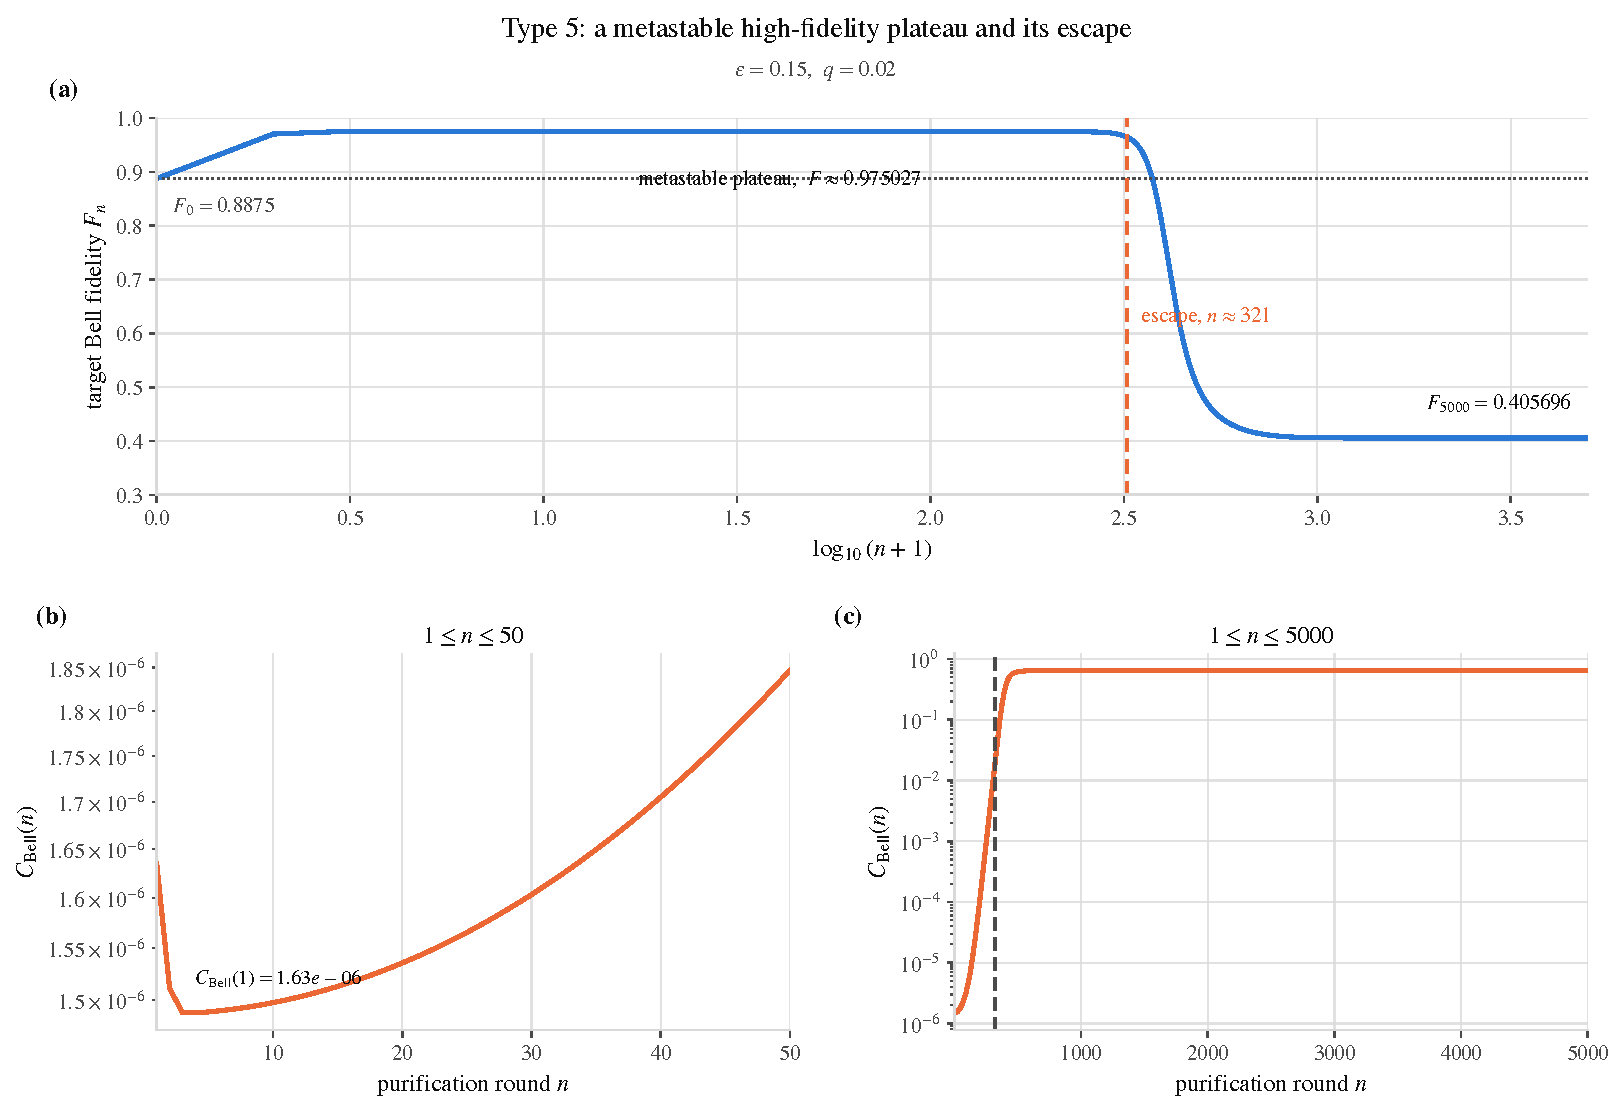
\includegraphics[width=0.90\linewidth]{figures/type5_metastability.pdf}\\[0.2ex]
    {\scriptsize\color{qitgray}Type 5: purify, plateau, escape.}\\[1.4ex]
    \raggedright\scriptsize
    \textbf{Headline.}\; The best one-round circuit is \emph{not} the best
    repeated one --- Type 5 has the smallest first-order loss and the worst
    long-run behaviour.
    \smallskip

    \unit{Scope: the Type 3/4/5 read-out is parity-\emph{weighted}, so
    iterating it is an effective nonlinear map, not a shot-by-shot protocol.}
  \end{column}
  \end{columns}
\end{frame}

% ===========================================================================
% 9. Resource comparison
% ===========================================================================
\begin{frame}{9 \quad Resource comparison}{What each protocol costs, and where the CNOT savings actually come from}
  \vspace{0.8ex}
  \centering\scriptsize\renewcommand{\arraystretch}{1.05}%
  \setlength{\tabcolsep}{3.6pt}
  \begin{tabular}{@{}l c c c l l c@{}}
    \toprule
    & qubits & CNOTs & cross-party & output & per-round cost & Bell-diag.\ closure\\
    \midrule
    \textbf{4Q} comparator   & 4 & \acc{5}  & 3 & a physical state  & $P_{\mathrm{succ}}=\Tr\rho^{2}$ & yes\\\rowgap
    \textbf{5Q} Type 3       & 5 & 16 & --- & expectation value & sampling overhead & yes\\\rowgap
    \textbf{5Q} Type 4       & 5 & 14 & --- & expectation value & sampling overhead & yes\\\rowgap
    \textbf{5Q} Type 5       & 5 & 14 & --- & expectation value & sampling overhead & \warn{no}\\\rowgap
    \textbf{6Q}-L16          & 6 & 16 & \acc{0} & expectation value & sampling overhead & yes\\\rowgap
    \textbf{6Q}-L14          & 6 & 14 & \acc{0} & expectation value & sampling overhead & yes\\\rowgap
    destructive VD \unit{(reference)} & 4 & \acc{2} & --- & $\avg{O}$ per measurement setting & many settings & n/a\\
    \bottomrule
  \end{tabular}

  \vspace{2.4ex}
  \begin{columns}[T,onlytextwidth]
  \begin{column}{0.43\textwidth}\vspace{0pt}
    \scriptsize
    \textbf{Where the savings come from}
    \smallskip

    \begin{tabular}{@{}l c@{}}
      \toprule
      circuit must reproduce & min.\ CNOTs\\
      \midrule
      the full unitary $U$            & \textbf{14} \unit{(13 unreachable)}\\\rowgap
      the ancilla-$\ket{0}$ isometry  & \textbf{14} \unit{(no gain)}\\\rowgap
      the observable, parity read-out & \textbf{5}\\\rowgap
      the observable, destructive read-out & \textbf{2}\\
      \bottomrule
    \end{tabular}
    \smallskip

    \acc{Every saving comes from relaxing the observable}; relaxing unitary
    to isometry buys nothing.
  \end{column}
  \begin{column}{0.53\textwidth}\vspace{0pt}
    \scriptsize
    \textbf{One-round threshold $\varepsilon_2^{*}$ --- placement, not count}
    \smallskip

    \begin{tabular}{@{}l c c c c@{}}
      \toprule
      input $\varepsilon$ & Type 3 (16) & Type 4 (14) & Type 5 (14) & destructive (2)\\
      \midrule
      0.10 & 0.033 & 0.041 & \acc{0.060} & 0.146\\\rowgap
      0.40 & 0.103 & 0.140 & \acc{0.237} & 0.313\\\rowgap
      0.60 & 0.126 & 0.178 & \acc{0.338} & 0.343\\
      \bottomrule
    \end{tabular}
    \smallskip

    $16\to14$ buys $1.25$--$1.42\times$, more than the ratio $1.14$; two
    \emph{exact} 14-CNOT implementations differ by $1.5$--$1.9\times$.
    \textbf{$\Rightarrow$ count, depth and noiseless fidelity do not
    characterise a noisy PQEC circuit.}
  \end{column}
  \end{columns}
\end{frame}

% ===========================================================================
% 10. Operational thresholds -- definitions
% ===========================================================================
\begin{frame}{10 \quad Operational thresholds}{Five inequivalent questions hide behind ``the threshold''}
  \vspace{0.8ex}
  \scriptsize
  Target $\Phip$;\;
  $p_i^{(n)}=\bra{B_i}\rho_n\ket{B_i}$,\;
  $R_i^{(n)}=p_i^{(n)}/p_{\Phip}^{(n)}$,\;
  $F_n=\bra{\Phip}\rho_n\ket{\Phip}$.
  \smallskip

  \setlength{\tabcolsep}{4pt}\begin{tabular}{@{}l l p{0.45\textwidth} l@{}}
    \toprule
    & & predicate & what it certifies\\
    \midrule
    1 & $q_{\mathrm{abs}}$   & $p_i^{(n+1)}<p_i^{(n)}$ for every non-target $i$ and every $n\ge0$ & every Bell error population falls\\\rowgap
    2 & $q_{\mathrm{rel}}$   & $R_i^{(n+1)}<R_i^{(n)}$ for every non-target $i$ and every $n$ & errors fall \emph{relative} to the target\\\rowgap
    3 & $q_{\mathrm{th}}$    & $F_{n+1}>F_n$ for every $n\ge0$ & the fidelity really improves\\\rowgap
    4 & $q_{\mathrm{fixed}}$ & the target fixed point exists \unit{(saddle node, discriminant $=0$)} & repetition converges somewhere useful\\\rowgap
    5 & $q_{\mathrm{target}}$& the target fixed point still has $F_\star>1/2$ & the limit is still entangled\\
    \bottomrule
  \end{tabular}

  \vspace{2.6ex}
  \begin{columns}[T,onlytextwidth]
  \begin{column}{0.46\textwidth}\vspace{0pt}
    \scriptsize
    \textbf{Prior work's criterion}\\[0.3ex]
    $F_{\mathrm{out}}>F_{\mathrm{bare}}$, \emph{one} round, noise on the data
    only --- the $n=0$ case of (3), kept separate as a diagnostic:
    \begin{align*}
      q_{\mathrm{th}}^{\mathrm{first}}&=\sup\{q: F_1>F_0\}\\
      \text{vs.}\quad
      q_{\mathrm{th}}^{\mathrm{full}}&=\sup\{q: F_{n+1}>F_n\;\forall n\}.
    \end{align*}
    Whether the two coincide is an \emph{output}, not an assumption.
  \end{column}
  \begin{column}{0.50\textwidth}\vspace{0pt}
    \scriptsize
    \textbf{Rules we imposed on ourselves}
    \begin{itemize}\itemsep0.3ex
      \item measured from the \emph{full} noisy circuit: no analytic
            recurrence, no closed-form map, no invariant-plane projection,
            no twirling;
      \item no previously measured threshold used as a bracket or hint;
      \item two independent implementation routes (agreeing to
            $1.7\times10^{-15}$) plus a 400-bit ball-arithmetic route;
      \item orderings and rankings compared only \emph{after} the primary
            tables were frozen.
    \end{itemize}
  \end{column}
  \end{columns}
\end{frame}

% ===========================================================================
% 11. Threshold results
% ===========================================================================
\begin{frame}{11 \quad Threshold results}{Circuit-level numerics: 39 $(\text{protocol},\varepsilon)$ points, 37 bisected to $7.45\times10^{-11}$}
  \vspace{0.6ex}
  \begin{columns}[T,onlytextwidth]
  \begin{column}{0.50\textwidth}\vspace{0pt}
    \centering
    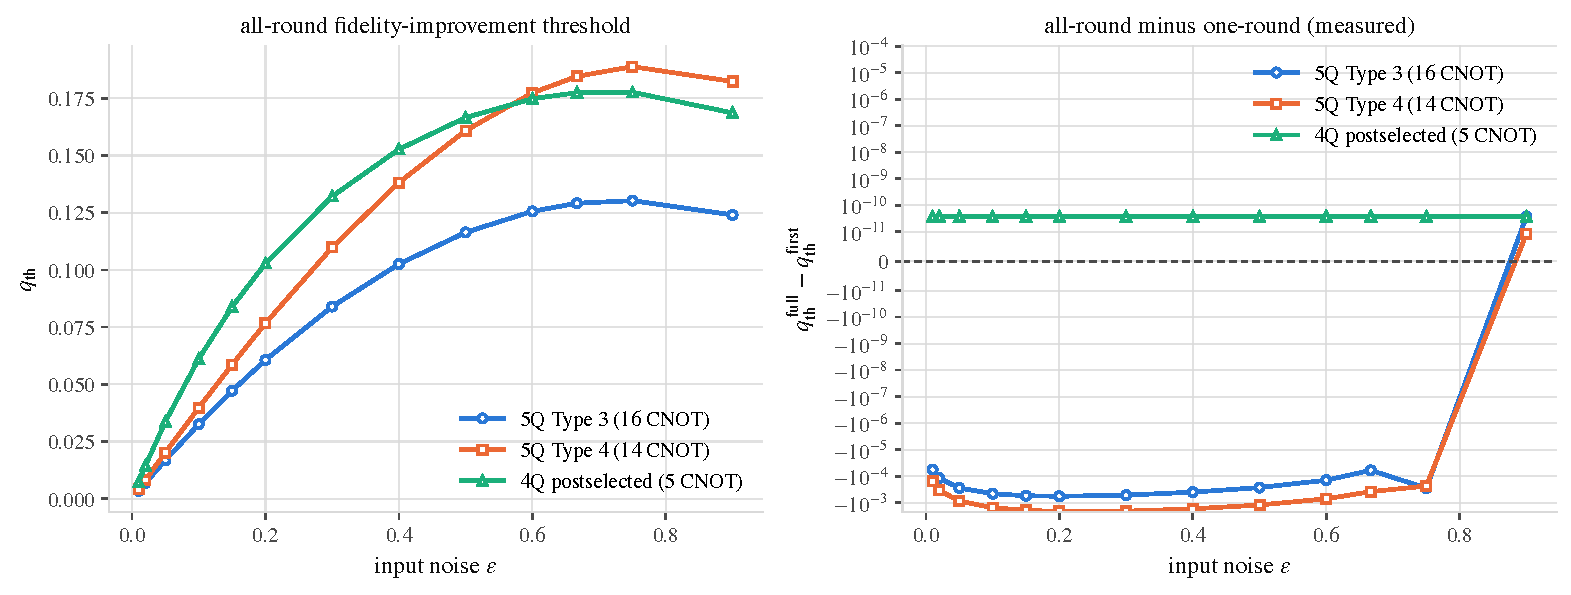
\includegraphics[width=\linewidth]{figures/qth_curves.pdf}\\[1.2ex]
    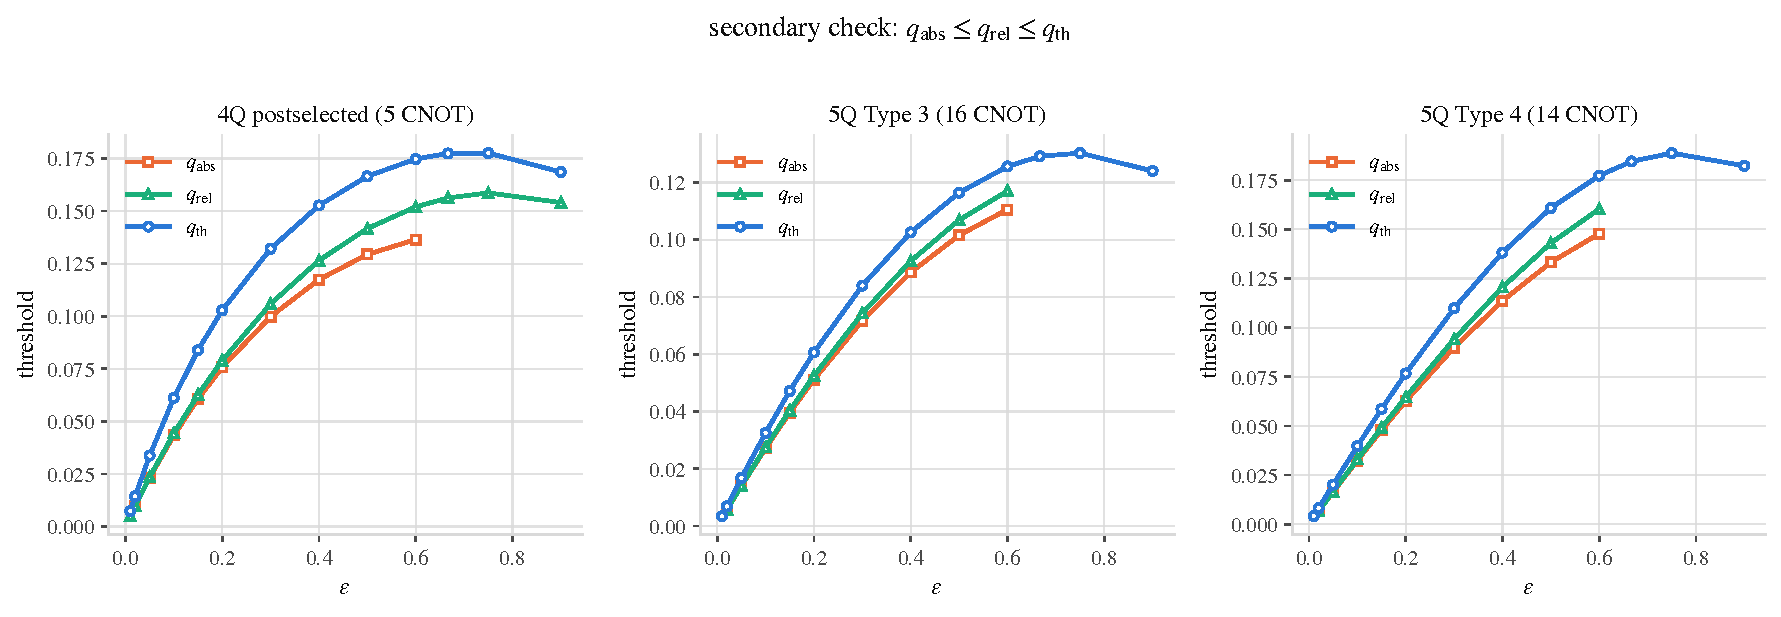
\includegraphics[width=0.97\linewidth]{figures/qth_hierarchy.pdf}
  \end{column}
  \begin{column}{0.46\textwidth}\vspace{0pt}
    \scriptsize
    \textbf{(a) The hierarchy holds at all 39 points} \stat{numerical}
    \smallskip

    \begin{tabular}{@{}l c c c@{}}
      \toprule
      $\varepsilon=0.40$ & $q_{\mathrm{abs}}$ & $q_{\mathrm{rel}}$ & $q_{\mathrm{th}}$\\
      \midrule
      Type 3 & 0.08857 & 0.09253 & 0.10255\\\rowgap
      Type 4 & 0.11364 & 0.12058 & 0.13815\\\rowgap
      4Q     & 0.11740 & 0.12651 & 0.15269\\
      \bottomrule
    \end{tabular}
    \smallskip

    \textbf{(b) All-round vs.\ one-round --- protocol dependent}
    \begin{itemize}\itemsep0.2ex
      \item \textbf{4Q}: equal at every $\varepsilon$ to
            $7.45{\times}10^{-11}$; binding round \acc{0}.
      \item \textbf{Type 3 / 4}: \warn{strictly smaller}, by
            $6{\times}10^{-5}\ldots2.2{\times}10^{-3}$; the binding round
            grows with $\varepsilon$ to \acc{28} and \acc{36}.
      \item \textbf{107} trajectories rise, then turn over; \textbf{0} do
            the opposite.
    \end{itemize}
    \medskip

    \textbf{(c) The ranking crosses between $\varepsilon=0.50$ and
    $0.60$}\\[0.3ex]
    4Q $>$ T4 $>$ T3 \;$\longrightarrow$\; \acc{T4} $>$ 4Q $>$ T3.\;
    Maxima near $\varepsilon=0.75$: $0.1888$ / $0.17759$ / $0.13024$.
    \smallskip

    {\color{qitink2}\textbf{Caveat.} The Type 3/4 all-round threshold is set
    by a \emph{late-round} dip, so it carries a tolerance dependence of
    $10^{-7}$--$10^{-6}$ --- digits past the sixth are not physical. The gap
    to $q_{\mathrm{th}}^{\mathrm{first}}$ is $10^{2}$--$10^{4}$ larger, so
    the inequality stands.}
  \end{column}
  \end{columns}
\end{frame}

% ===========================================================================
% 12. Discussion and next steps
% ===========================================================================
\begin{frame}{12 \quad Discussion and next steps}{What is settled, what is open, what the paper needs}
  \vspace{0.8ex}
  \scriptsize
  \begin{columns}[T,onlytextwidth]
  \begin{column}{0.46\textwidth}\vspace{0pt}
    \textbf{Settled}
    \begin{itemize}\itemsep0.25ex
      \item exact noisy Bell-diagonal maps and fixed points for 4Q,
            Type 3, Type 4, with \acc{$q_{\mathrm{SN}}$,
            $q_{\mathrm{ent}}$} in closed form;
      \item Fredkin-level depolarizing is self-mitigating --- the threshold
            lives in the \emph{decomposition};
      \item the 14-CNOT Type-4 circuit factorises into two
            $e^{-i\pi/8}\!\times\!$Fredkin blocks, defining 6Q-L14;
      \item 5Q\,$\equiv$\,6Q as estimators \emph{with the noise included}:
            proved for Type 3 and Type 4, arbitrary $R$, $O$, $q$;
      \item $q_{\mathrm{abs}}\le q_{\mathrm{rel}}\le q_{\mathrm{th}}$
            everywhere tested, and $q_{\mathrm{th}}^{\mathrm{full}}<
            q_{\mathrm{th}}^{\mathrm{first}}$ for Type 3/4.
    \end{itemize}
    \smallskip

    \textbf{Open --- analytic}
    \begin{itemize}\itemsep0.15ex
      \item a closed form for $q_{\mathrm{th}}(\varepsilon)$, for any
            protocol;
      \item why all-round and one-round thresholds coincide for 4Q but
            strictly not for Type 3/4, and where the binding round
            returns to 0;
      \item how far that equality survives once the ancilla-block
            closure is broken (mixing syntheses, asymmetric noise, noisy
            6Q read-out);
      \item a symbolic proof of the Type 3/4 two-sided Pauli covariance
            for all $q$.
    \end{itemize}
  \end{column}
  \begin{column}{0.50\textwidth}\vspace{0pt}
    \textbf{Open --- Type 5 and the full state}
    \begin{itemize}\itemsep0.25ex
      \item a fully symbolic derivation of the product fixed \emph{circle}
            (now semi-analytic,
            $\|M(\rho_\star)-\rho_\star\|_F\sim10^{-10}$);
      \item a complete classification of fixed points and basins --- the
            circle is only the observed asymptotic family;
      \item is it the $R_X,R_Y,R_Z$ layers themselves that break the
            symmetry, or only this learned placement?
    \end{itemize}
    \medskip

    \textbf{Next circuits and noise models}
    \begin{itemize}\itemsep0.25ex
      \item Cruz--Murta 7-CNOT Fredkin (arXiv:2305.18128) and
            Smolin--DiVincenzo five two-qubit gates (PRA \textbf{53}, 2855)
            in the same CNOT-only model;
      \item coherent and biased CNOT errors;
      \item entanglement-based thresholds (concurrence, negativity) and
            their multi-round accumulation;
      \item 6Q-L14 / 6Q-L16 under \emph{asymmetric} party noise.
    \end{itemize}
    \medskip

    \textbf{For the paper}\; freeze the protocol table and the three
    threshold tables; fold the two equivalence proofs in as lemmas;
    one figure set, one reproducibility appendix.
  \end{column}
  \end{columns}
\end{frame}

\end{document}
